\section{Skica uživatelského rozhraní}\label{sec:ui}

Systém má dvě uživatelská rozhraní. \textbf{Desktopová aplikace (JavaFX)} slouží pracovníkům a administrátorovi a realizuje případy užití \ucref{02}, \ucref{08}, \ucref{13}, \ucref{16}, \ucref{19} a pracovníkovu část \ucref{11} (sdílení). \textbf{Webové rozhraní} slouží zákazníkům a realizuje zákazníkovu část \ucref{11} (zobrazení nabídky a komentář). Manažerům slouží webové rozhraní po přihlášení k prohlížení projektů (\ucref{15}). Tato část rozhraní není podrobně popsána.

Díky oddělení vrstev volají obě rozhraní stejné aplikační služby.

Náčrty ukazují zamýšlený vzhled obrazovek s ukázkovými daty jedné zakázky (projekt Svatba Novákových, revize 3 svatebního menu). Všechny obrazovky používají stejná data, aby na sebe navazovaly.

U každé obrazovky je uvedeno, které kroky případu užití na ní probíhají (například \uv{UC02/3} znamená krok 3 případu užití \ucref{02}). Přehled přechodů mezi obrazovkami je v tabulce~\ref{tab:prechody}.

\subsection{Vizuální styl a realizovatelnost}

Obě rozhraní sdílejí jeden jednoduchý vizuální styl. Pozadí je světle šedé a obsah leží na bílých kartách se zaoblenými rohy. Hlavní akce na obrazovce má vždy jediné tlačítko v akcentní barvě (tmavě tyrkysová), ostatní tlačítka jsou obrysová.

Stavy objektů (ROZPRACOVANÝ, PRACOVNÍ, SDÍLENÁ, NEVYŘÍZENÝ, VYŘÍZENÝ, Aktivní) se zobrazují jako barevné štítky, které mají kromě barvy i text, takže je rozliší i člověk s poruchou barevného vidění.

Chyby ve formuláři se ukazují přímo u pole, kterého se týkají. Chyby celé operace (například příliš velký soubor nebo položku, kterou nelze smazat) ohlásí dialogové okno. Důležité upozornění (například jen pro čtení) je barevný pruh nad obsahem, případně s tlačítkem, které situaci vyřeší.

Návrh záměrně používá jen prvky, které nabízí standardní JavaFX a obyčejné HTML s CSS bez dalších knihoven (kromě knihovny ZXing pro QR kód). Vzhled desktopové aplikace určuje jeden soubor stylů \texttt{app.css} (vlastnosti \texttt{-fx-background-color}, \texttt{-fx-background-radius}, \texttt{-fx-border-color} a efekt \texttt{dropshadow}).

Webové stránky generuje server jako čisté HTML s jedním souborem \texttt{web.css} a nepotřebují JavaScript.

Ikony jsou jednoduché obrysové tvary, které se v JavaFX kreslí uzlem \texttt{SVGPath} a na webu prvkem \texttt{svg}. Tabulka~\ref{tab:prvky} ukazuje, čím se jednotlivé prvky náčrtů realizují.

\begin{table}[H]
\centering
\small
\begin{tabularx}{\textwidth}{lXX}
\toprule
\textbf{Prvek náčrtu} & \textbf{JavaFX} & \textbf{Web (HTML a CSS)} \\
\midrule
Rozvržení obrazovky & \texttt{BorderPane}, \texttt{SplitPane}, \texttt{VBox}, \texttt{HBox} & \texttt{div} s \texttt{display:flex} \\
Seznam komentářů & \texttt{ListView} s vlastní buňkou (\texttt{ListCell}) & seznam prvků \texttt{div} \\
Strom obsahu projektu & \texttt{TreeView} & \\
Obsah aktivní složky & \texttt{TableView} se sloupcem \texttt{CheckBox} & \\
Výběr souboru a cílové složky & \texttt{FileChooser}, \texttt{DirectoryChooser} & \\
Tabulka položek a uživatelů & \texttt{TableView}, úprava v buňce \texttt{TextFieldTableCell} & \texttt{table} \\
Stavový štítek & \texttt{Label} se stylem \texttt{.chip} & \texttt{span} s třídou \texttt{chip} \\
Upozorňující pruh & \texttt{HBox} se stylem \texttt{.banner} & \texttt{div} s třídou \texttt{banner} \\
Výběr projektu, zákazníka a revize & \texttt{ComboBox} & \\
Výběr položky \uv{Týká se} & & \texttt{select} \\
Datum akce & \texttt{DatePicker} & \\
Záložky Nevyřízené, Vyřízené a Vše & \texttt{TabPane} nebo \texttt{ToggleButton} ve skupině & \\
Role a aktivní účet & \texttt{CheckBox}, \texttt{ToggleButton} & \\
Dialogy \odkaz{scr:D2}{D2}, \odkaz{scr:D3}{D3}, \odkaz{scr:D6}{D6}, \odkaz{scr:D8}{D8} & \texttt{Dialog} nebo modální \texttt{Stage} & \\
Formulář komentáře & & \texttt{form} s metodou POST \\
QR kód & \texttt{ImageView} s obrázkem vytvořeným knihovnou ZXing & \texttt{img} \\
\bottomrule
\end{tabularx}
\caption{Realizace prvků náčrtů v JavaFX a ve webovém rozhraní}
\label{tab:prvky}
\end{table}

\subsection{Desktopová aplikace}

\phantomsection\label{scr:D1}
\subsubsection*{D1 -- Hlavní okno}
\begin{figure}[H]
  \centering
  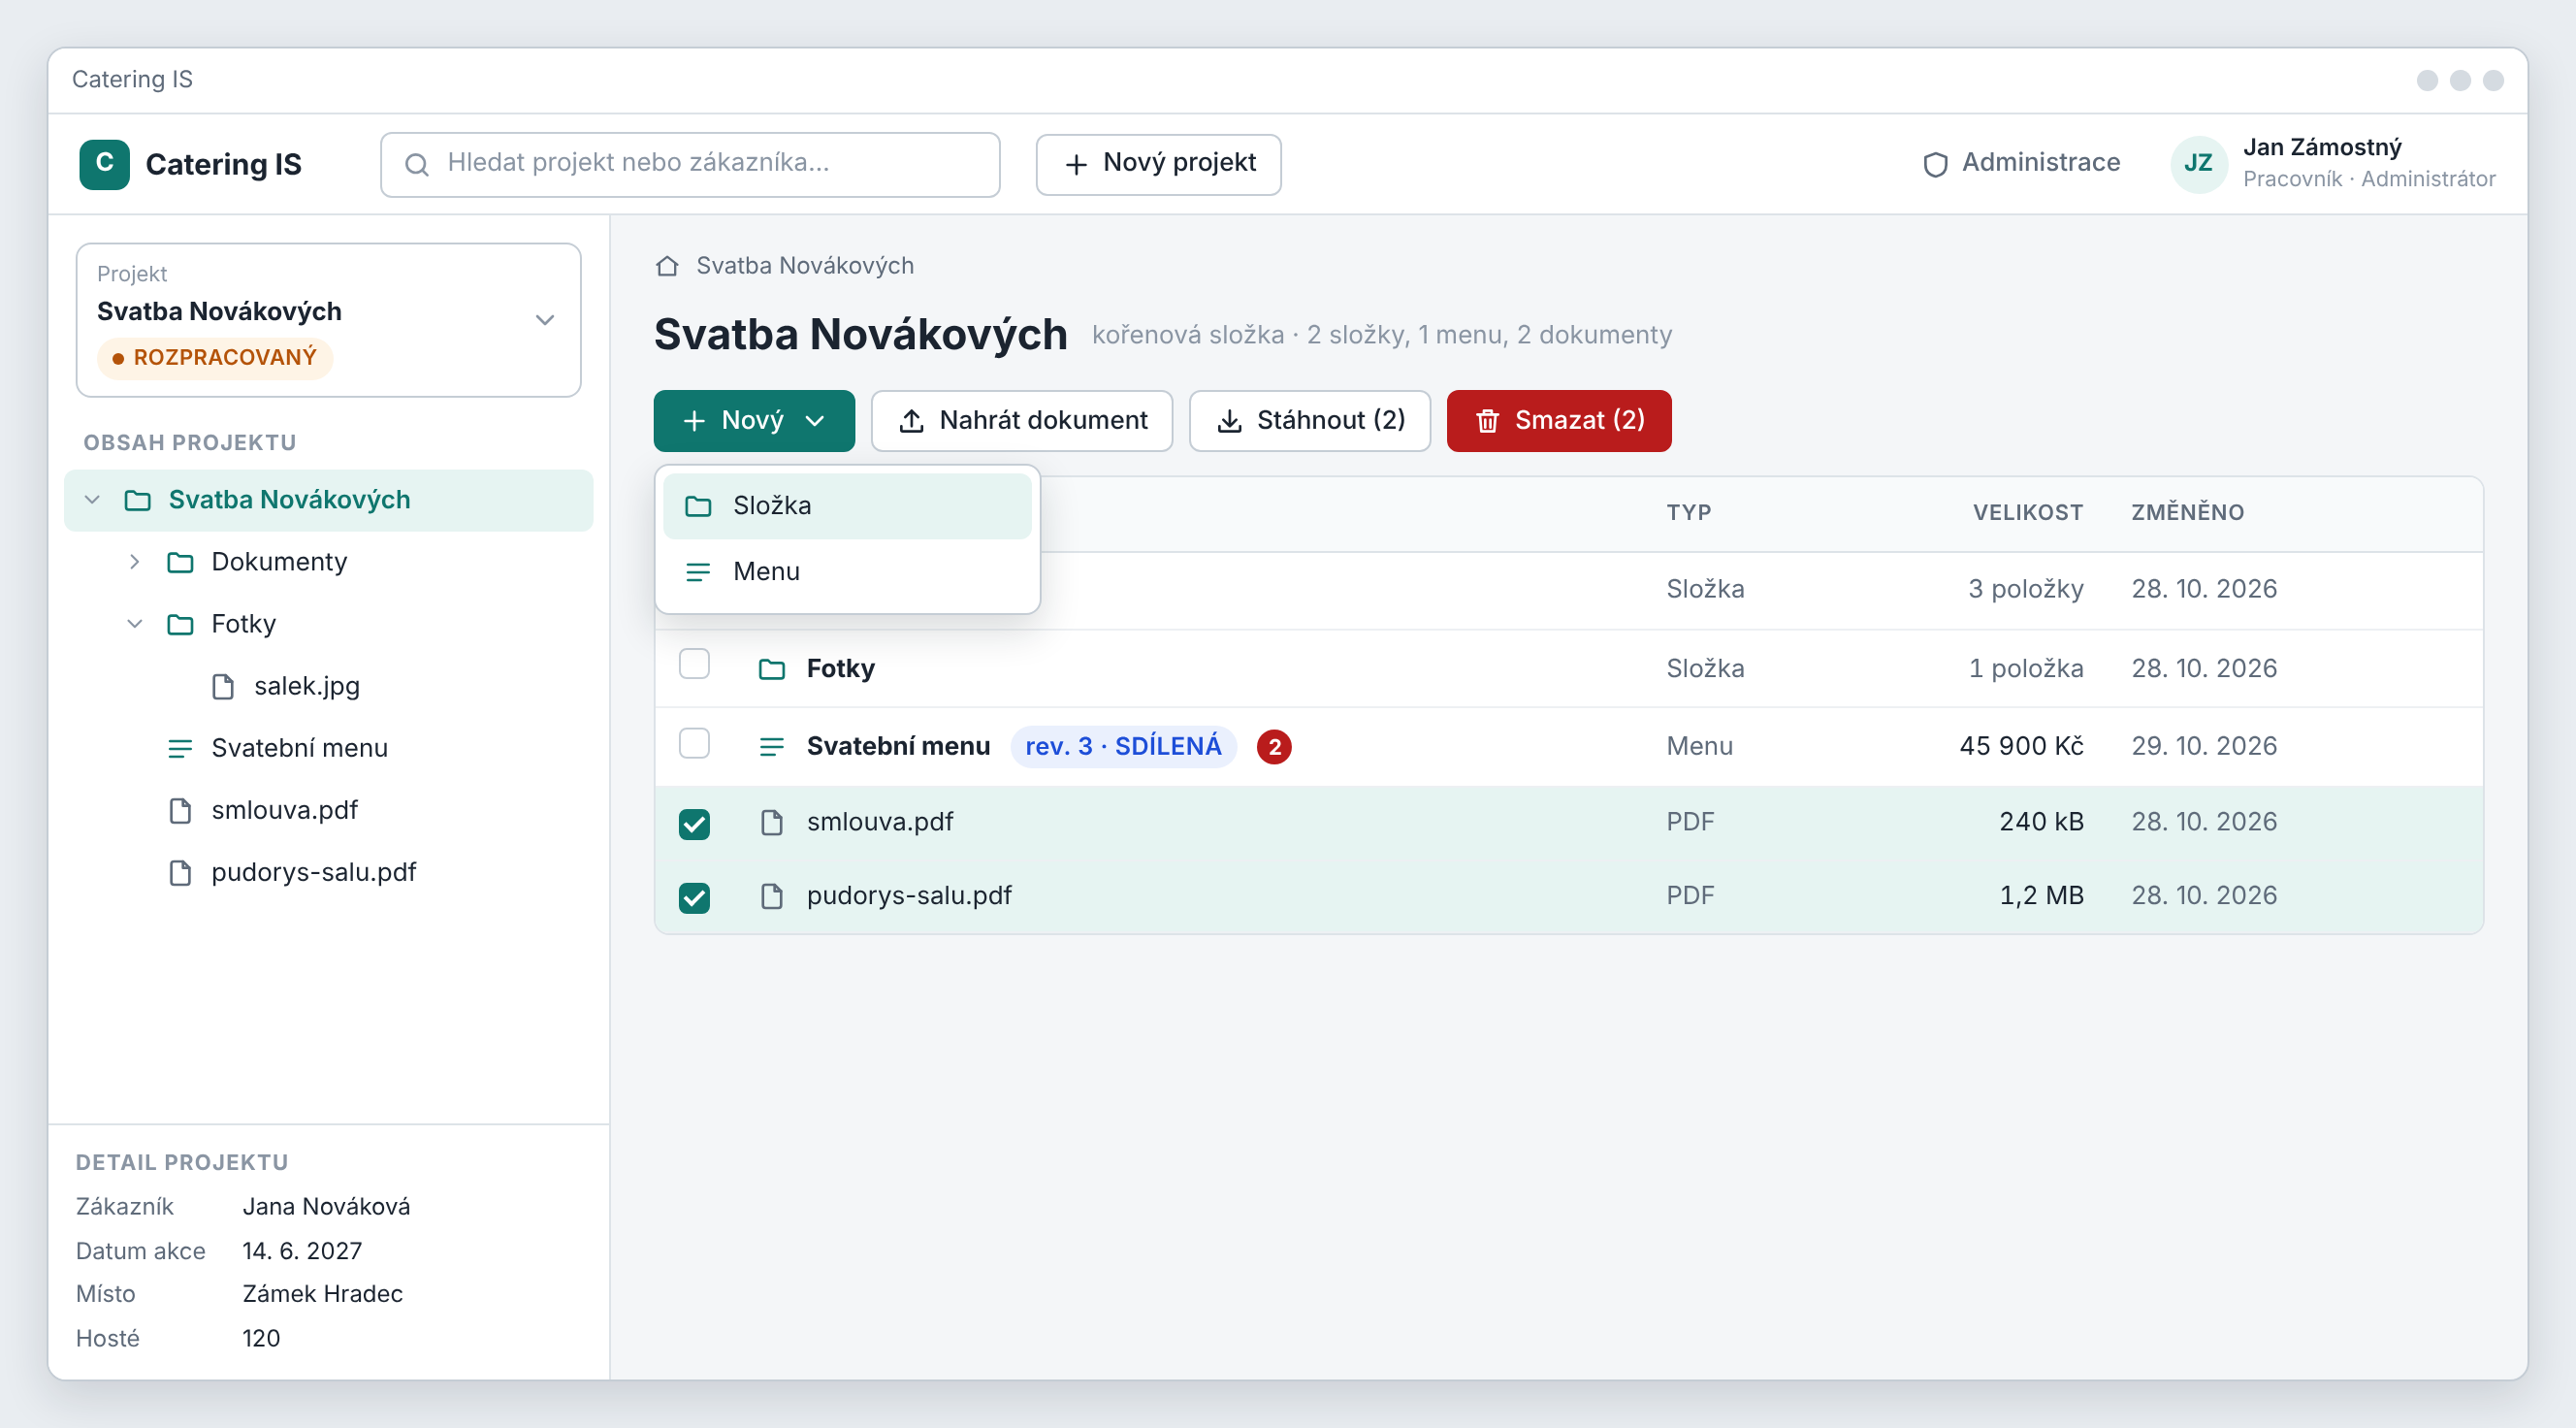
\includegraphics[width=\textwidth]{ui-main.png}
  \caption{D1 -- Hlavní okno desktopové aplikace}
  \label{fig:d1}
\end{figure}

Okno je jednoduchý průzkumník souborů projektu. V horní liště je vyhledávání projektů (\ucref{04}), tlačítko \uv{Nový projekt}, přihlášený uživatel se svými rolemi a tlačítko \uv{Administrátorský režim} pro přepnutí do administrátorského režimu (\ucref{17}), které je viditelné pouze aktivním administrátorům. Hlavní okno se zobrazí jen uživateli s rolí pracovníka, administrátor bez této role se dostane rovnou do administrátorského režimu (\odkaz{scr:D7}{D7}).

Levý sloupec obsahuje výběr projektu se stavem, pod ním strom obsahu projektu a dole stručný detail projektu s tlačítkem \uv{Upravit projekt} (\ucref{03}). Dialog úprav umožní projekt archivovat a před archivací se zeptá, pokud jsou v něm neuložené změny. U archivovaného projektu je dialog jen pro čtení a nabízí tlačítko \uv{Obnovit projekt}, které po potvrzení vrátí projekt do stavu ROZPRACOVANÝ. Archivovaný projekt je zcela jen pro čtení, tedy včetně vytváření položek, nahrávání, mazání a ukládání revizí menu. Strom funguje jako ve vývojovém prostředí. Složky lze rozbalit a sbalit. Kromě složek strom ukazuje i menu a dokumenty. Výběrem složky ve stromu se tato složka stane aktivní (\odkaz{uc:02:7}{UC02/7}).

Pravá část funguje jako běžný správce souborů a ukazuje obsah aktivní složky. Nad obsahem je cesta ke složce a její název. Tabulka uvádí podsložky, menu a dokumenty s typem, velikostí a datem změny.

U menu je číslo a stav revize, celková cena a počet nevyřízených komentářů zákazníka. Dvojklik otevře podsložku (\odkaz{uc:02:7}{UC02/7}) nebo menu v editoru \odkaz{scr:D4}{D4} (\odkaz{uc:08:1}{UC08/1}). Každý řádek tabulky má zaškrtávací políčko pro výběr položek.

Nad tabulkou jsou čtyři tlačítka. Nové položky se vytvářejí v aktivní složce.

\begin{itemize}[itemsep=2pt]
  \item \textbf{Nový} otevře nabídku s typy nových položek (\texttt{MenuButton}), jak ukazuje obrázek~\ref{fig:d1}. Nyní obsahuje volby \uv{Složka} a \uv{Menu}. Další typy, například jmenovky nebo jiné exportovatelné soubory, lze později přidat jako novou položku nabídky bez změny rozvržení okna.
  \begin{itemize}[itemsep=1pt]
    \item Volba \uv{Složka} vytvoří podsložku (\odkaz{uc:02:5}{UC02/5}). Pokud složka se stejným názvem již existuje, systém nabídne přejmenování v dialogu z obrázku \odkaz{fig:d3}{D3} (\odkaz{uc:02:6.1}{UC02/6.1}--6.2).
    \item Volba \uv{Menu} otevře jednoduchý dialog pro zadání názvu (\texttt{TextInputDialog}). Systém ověří, že název ve složce ještě není (\odkaz{uc:02:8}{UC02/8}), vytvoří menu s prázdnou první revizí ve stavu PRACOVNÍ a zobrazí je ve stromu i v obsahu složky (\odkaz{uc:02:9}{UC02/9}). Menu pak pracovník otevře a sestaví v editoru \odkaz{scr:D4}{D4} (\odkaz{uc:02:10}{UC02/10}).
  \end{itemize}
  \item \textbf{Nahrát dokument} otevře systémový dialog pro výběr souboru (\odkaz{uc:02:7.1}{UC02/7.1}--7.2). Soubor větší než 20~MB systém odmítne chybovým oknem s povolenou velikostí (\odkaz{uc:02:7.4}{UC02/7.4}), jinak dokument uloží a zobrazí v obsahu složky (\odkaz{uc:02:7.6}{UC02/7.6}--7.7).
  \item \textbf{Stáhnout} ukazuje počet vybraných dokumentů a je aktivní jen tehdy, když jsou vybrány pouze dokumenty. Po stisku si pracovník zvolí cílovou složku v počítači a systém dokumenty uloží a ohlásí jejich počet (\odkaz{uc:02:7.8}{UC02/7.8}--7.12).
  \item \textbf{Smazat} je červené tlačítko s ikonou koše a smaže vybrané dokumenty, menu nebo prázdné složky (\ucref{19}, ve funkční specifikaci popsán jen stručně). Před smazáním se vždy zobrazí potvrzovací dialog \odkaz{scr:D8}{D8}.
\end{itemize}

\phantomsection\label{scr:D2}
\subsubsection*{D2 -- Nový projekt (\ucref{02})}

\begin{figure}[H]
  \centering
  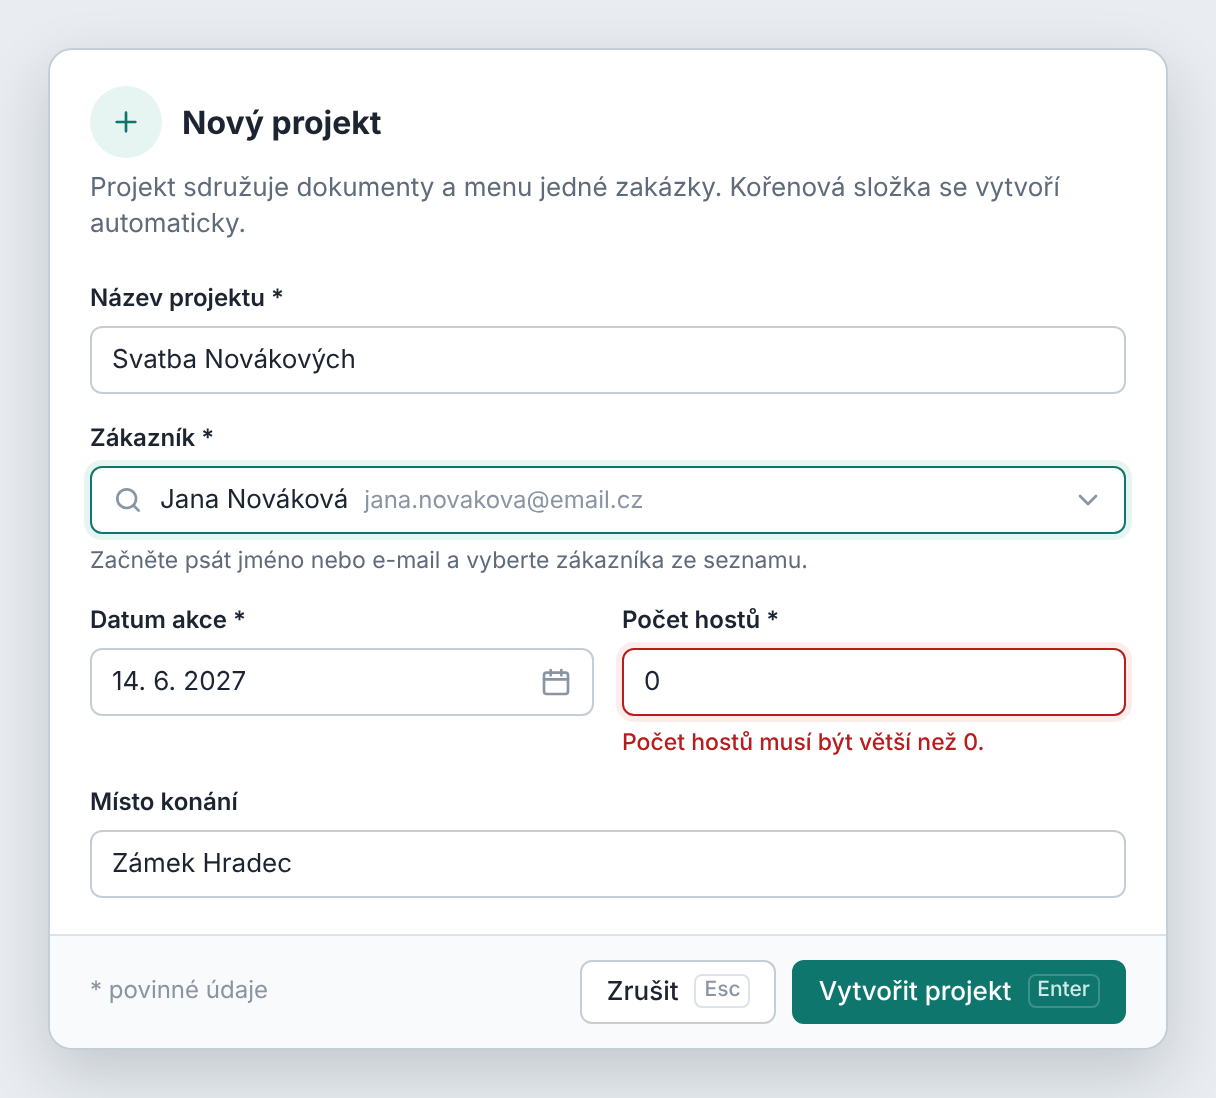
\includegraphics[width=0.62\textwidth]{ui-new-project.png}
  \caption{D2 -- Dialog nového projektu}
  \label{fig:d2}
\end{figure}

Dialog se otevře tlačítkem \uv{Nový projekt} v okně \odkaz{scr:D1}{D1} (\odkaz{uc:02:1}{UC02/1}--2).

Povinná pole jsou označena hvězdičkou. Zákazník se vybírá ze seznamu, ve kterém lze hledat podle jména i e-mailu. Datum se vybírá z kalendáře a počet hostů je celé číslo.

Po stisku \uv{Vytvořit projekt} (\odkaz{uc:02:3}{UC02/3}) systém údaje ověří. U chybného pole se objeví červený rámeček a pod ním popis chyby, jak ukazuje pole \uv{Počet hostů} na obrázku~\ref{fig:d2} (\odkaz{uc:02:4.1}{UC02/4.1}--4.3). Pokud jsou údaje v pořádku, dialog se zavře a nový projekt se zobrazí v okně \odkaz{scr:D1}{D1} s kořenovou složkou (\odkaz{uc:02:4}{UC02/4}).

Dialog lze ovládat i klávesnicí (Enter potvrdí, Esc zruší).

\phantomsection\label{scr:D3}
\subsubsection*{D3 -- Konflikt názvu (\ucref{02}, alternativní průběh)}

\begin{figure}[H]
  \centering
  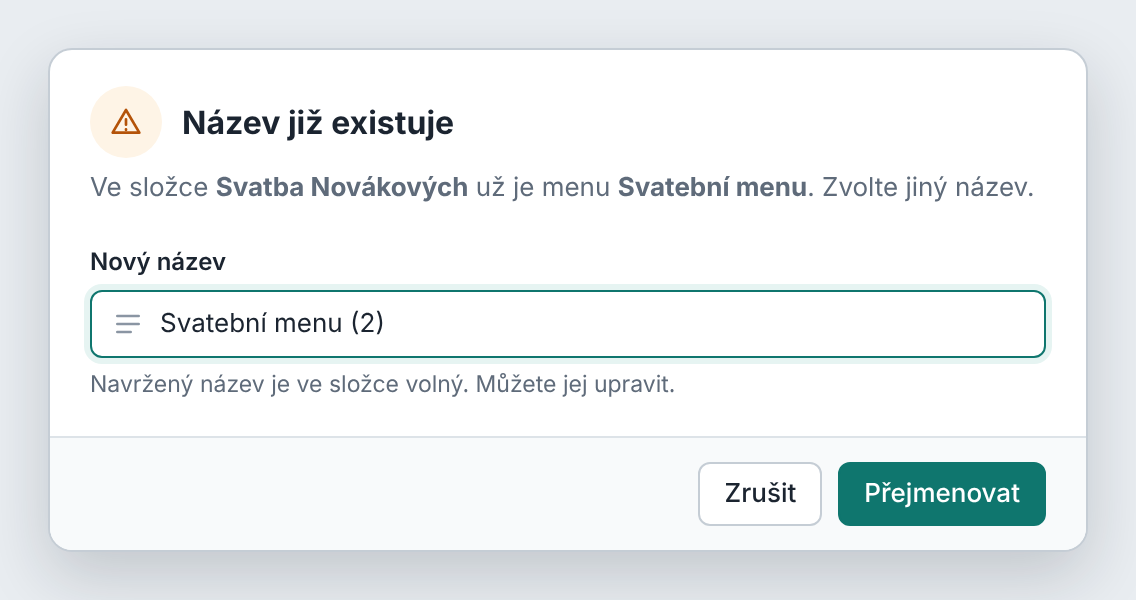
\includegraphics[width=0.6\textwidth]{ui-upload-conflict.png}
  \caption{D3 -- Dialog při existujícím názvu položky}
  \label{fig:d3}
\end{figure}

Dialog se zobrazí, pokud ve složce již existuje položka se stejným názvem (\odkaz{uc:02:8.1}{UC02/8.1}--8.5). Slouží pro oba způsoby vytvoření položky v okně \odkaz{scr:D1}{D1}: po zadání názvu nového menu i po výběru souboru tlačítkem \uv{Nahrát dokument} (\odkaz{uc:02:7.5}{UC02/7.5}).

Systém předvyplní nový název s pořadovým číslem, například \uv{Svatební menu (2)} nebo \uv{smlouva (2).pdf}. Pracovník název případně upraví a stiskne \uv{Přejmenovat}. Systém znovu ověří, že je název volný, a pokračuje vytvořením položky. Tlačítko \uv{Zrušit} vytvoření položky ukončí.

\phantomsection\label{scr:D4}
\subsubsection*{D4 -- Editor menu (\ucref{08}, \ucref{11}, \ucref{13})}
\begin{figure}[H]
  \centering
  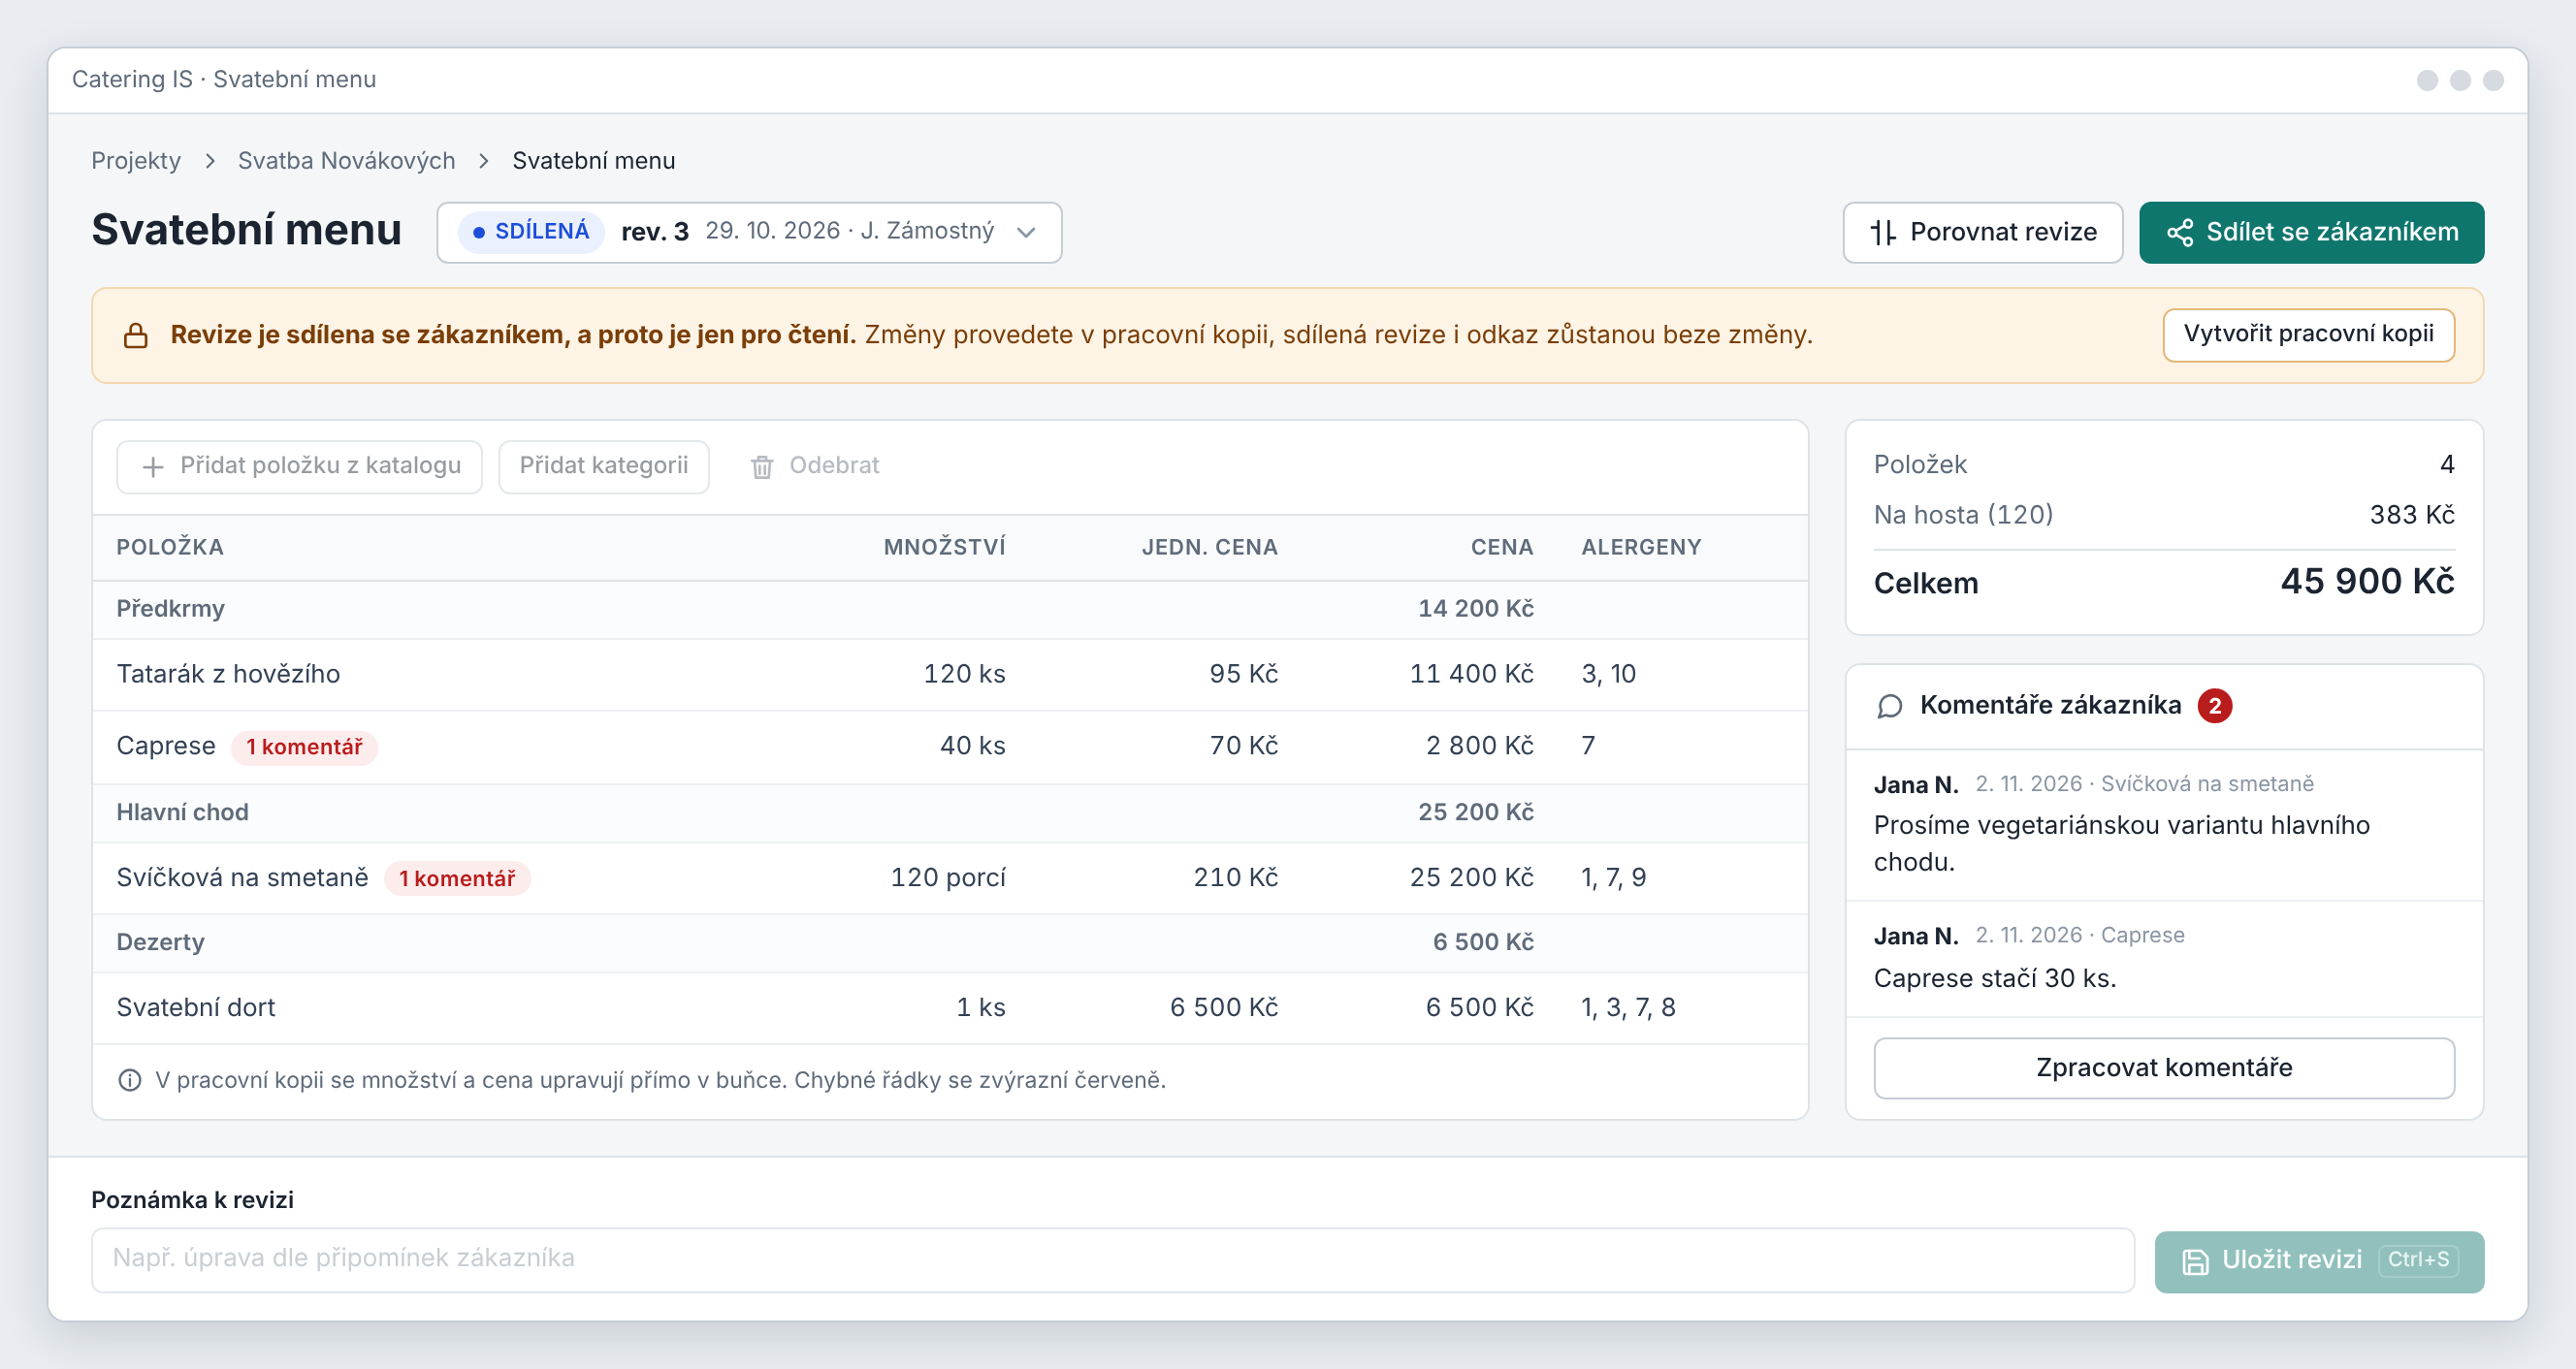
\includegraphics[width=\textwidth]{ui-menu-editor.png}
  \caption{D4 -- Editor menu se sdílenou revizí}
  \label{fig:d4}
\end{figure}

V záhlaví je cesta k menu, název menu a výběr revize (\ucref{09}), který ukazuje stav, číslo, datum a autora revize. Vpravo jsou tlačítka \uv{Porovnat revize} (\ucref{10}) a \uv{Sdílet se zákazníkem} (\odkaz{uc:11:1}{UC11/1}).

Je-li zobrazena sdílená revize, objeví se pod záhlavím žlutý pruh s vysvětlením a tlačítkem \uv{Vytvořit pracovní kopii} (\odkaz{uc:08:2.1}{UC08/2.1}--2.3). Tabulka a tlačítka pro úpravy jsou v tom případě neaktivní, jak ukazuje obrázek~\ref{fig:d4}.

Okno editoru se při neuložených změnách před zavřením zeptá, zda se mají změny zahodit. Po úpravách zůstane vybrán stejný řádek tabulky. Nad tabulkou jsou tlačítka \uv{Přidat položku z katalogu}, \uv{Přidat kategorii} a \uv{Odebrat} (\odkaz{uc:08:3}{UC08/3}). V pracovní kopii pracovník změní množství, cenu a poznámku položky tlačítkem \uv{Upravit položku} v dialogu (\ucref{08}, krok 3). Pole poznámky má popisek \uv{Poznámka (vidí zákazník)}, protože se poznámka zobrazuje zákazníkovi ve sdílené nabídce. Souhrn vpravo (počet položek, cena na hosta a celková cena) se přepočítá po každé změně (\odkaz{uc:08:4}{UC08/4}). Položky jsou seskupeny podle kategorií a řádek kategorie ukazuje její mezisoučet, který se také přepočítá po každé změně (\odkaz{uc:08:4}{UC08/4}). U položky, ke které zákazník napsal komentář, je červený štítek.

Dole je poznámka k revizi a tlačítko \uv{Uložit revizi} se zkratkou Ctrl+S (\odkaz{uc:08:5}{UC08/5}--8). Pracovní revize se přepíše a její číslo se nemění (\odkaz{uc:08:7}{UC08/7}). Pracovní kopie sdílené revize se uloží jako nová revize s číslem o jedna vyšším a sdílená revize zůstane beze změny (\odkaz{uc:08:2.5}{UC08/2.5}). Pokud je nejnovější revize už pracovní, systém pracovní kopii nevytvoří a zobrazí zprávu (\odkaz{uc:08:2.6}{UC08/2.6}--2.9). Pokud byla revize mezitím sdílena nebo už existuje novější revize, systém nic neuloží, zobrazí zprávu a načte nejnovější revizi (\odkaz{uc:08:7.1}{UC08/7.1}--7.3). Při neúspěšné kontrole se chybné řádky zvýrazní červeně a nic se neuloží (\odkaz{uc:08:6.2}{UC08/6.2}).

Vpravo pod souhrnem jsou komentáře zákazníka k revizi (výsledek \odkaz{uc:11:8}{UC11/8}) s počtem nevyřízených a tlačítkem \uv{Komentáře k rev. N (n nevyřízených)}, které otevře okno \odkaz{scr:D5}{D5} (\odkaz{uc:13:1}{UC13/1}).

\phantomsection\label{scr:D5}
\subsubsection*{D5 -- Zpracování komentářů (\ucref{13})}

\begin{figure}[H]
  \centering
  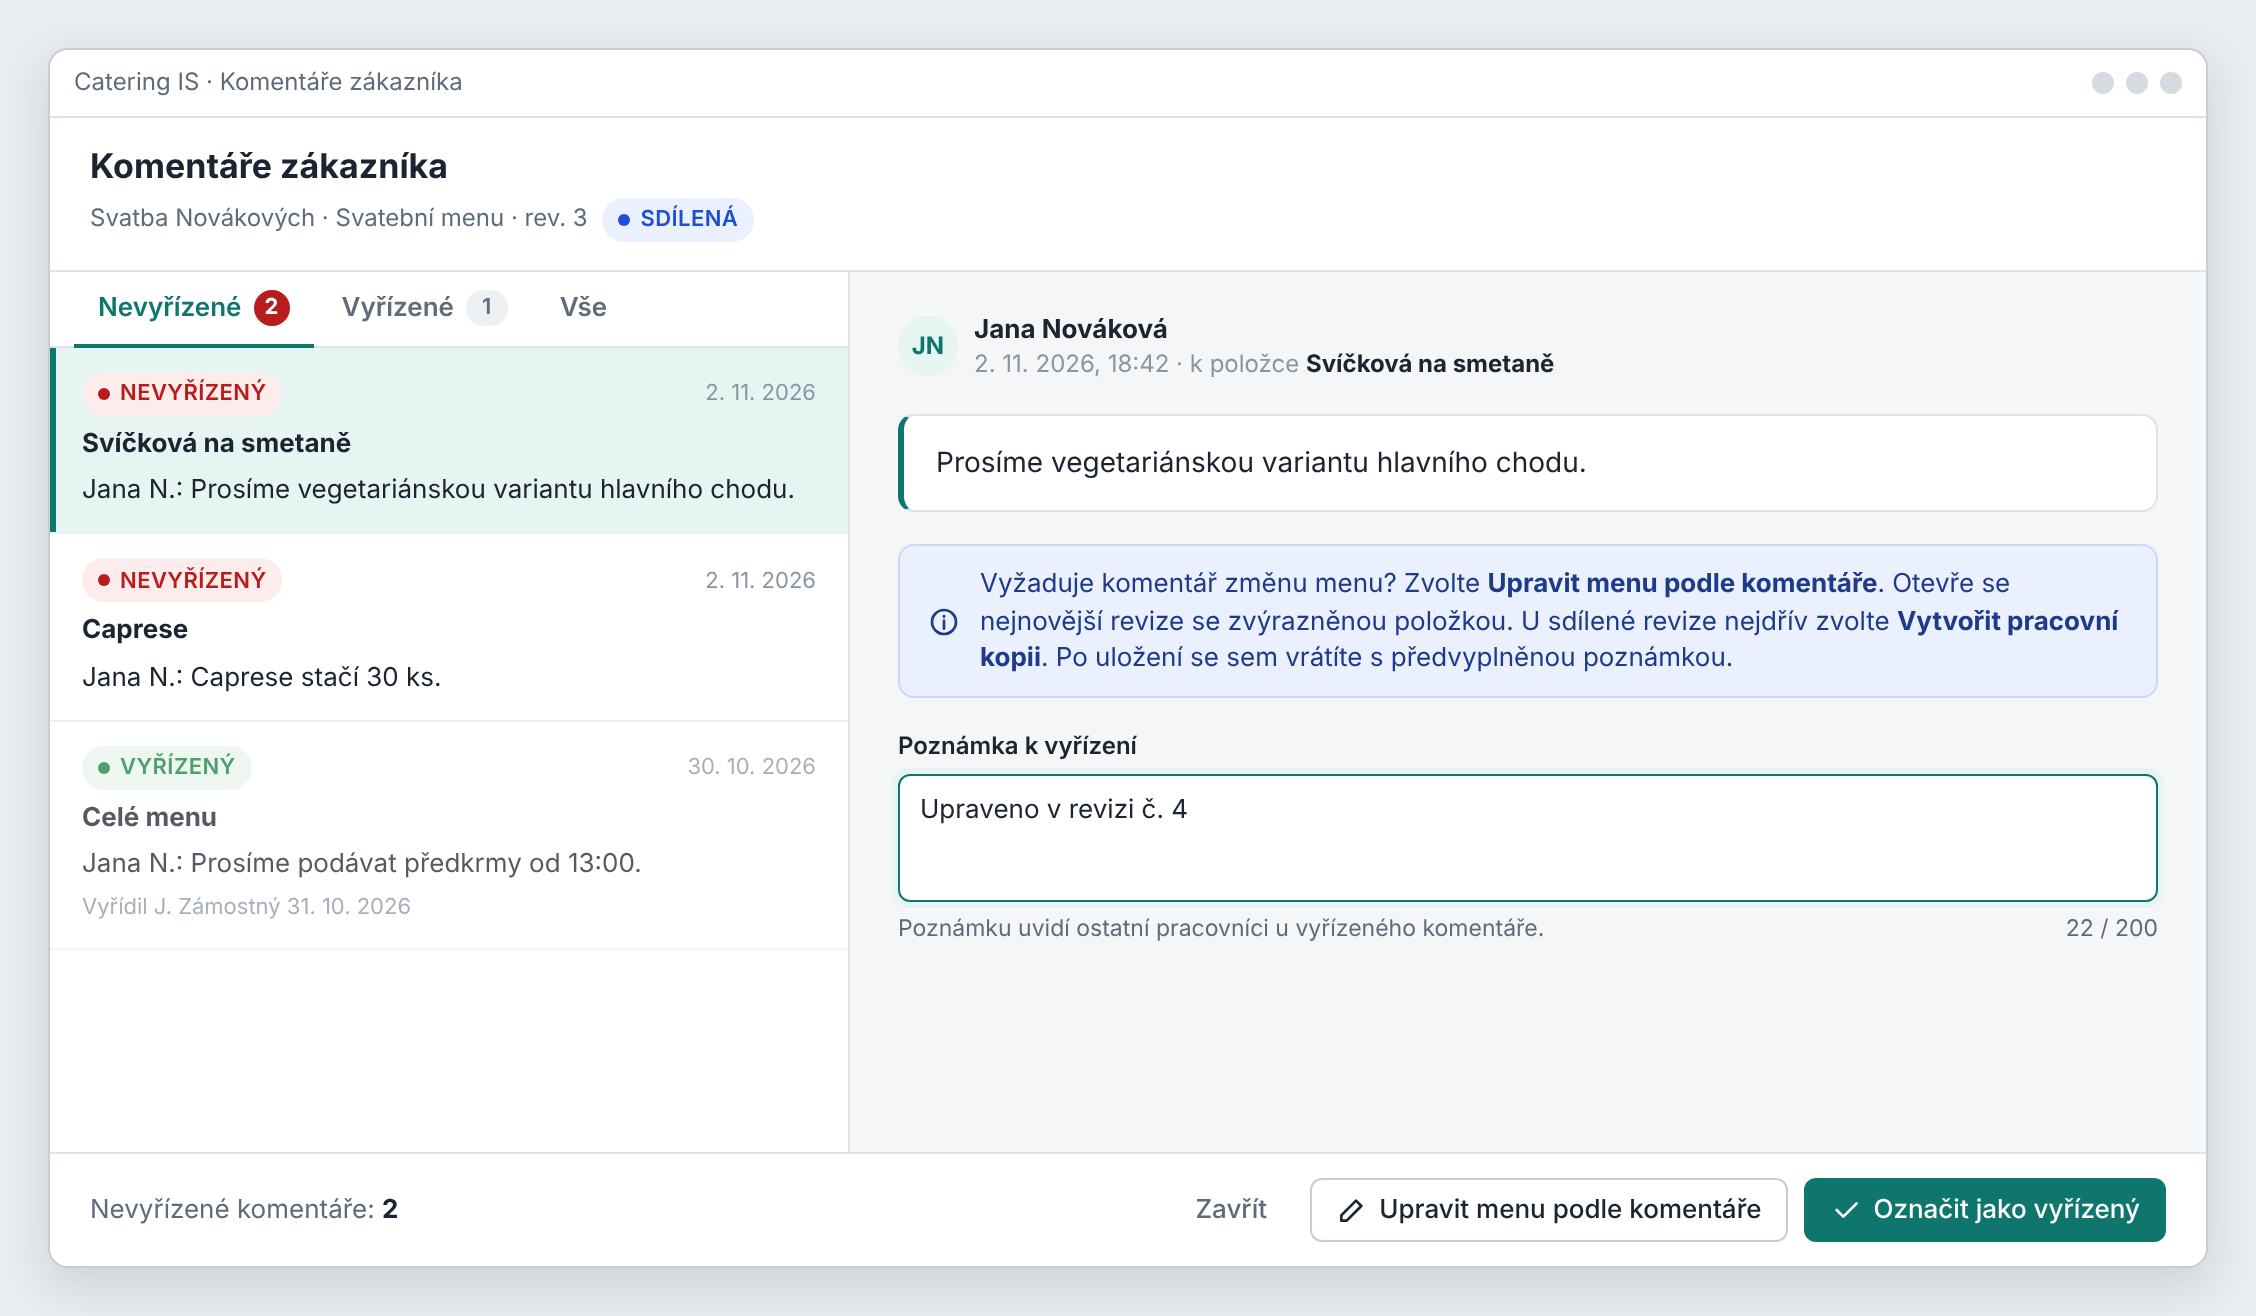
\includegraphics[width=\textwidth]{ui-comments.png}
  \caption{D5 -- Zpracování komentářů zákazníka}
  \label{fig:d5}
\end{figure}

Okno se otevře tlačítkem \uv{Komentáře k rev. N (n nevyřízených)} v editoru \odkaz{scr:D4}{D4} (\odkaz{uc:13:1}{UC13/1}--2).

Vlevo je seznam komentářů rozdělený na záložky Nevyřízené, Vyřízené a Vše, takže pracovník vidí nejdřív to, co čeká na vyřízení. U každého komentáře je stav, datum, položka menu a začátek textu. U vyřízeného komentáře je uvedeno, kdo a kdy jej vyřídil.

Vpravo je celý text vybraného komentáře, jeho autor a položka, ke které se vztahuje. Pracovník zapíše poznámku, která má nejvýše 200 znaků (pole ukazuje jejich počet), a stiskne \uv{Označit jako vyřízený} (\odkaz{uc:13:3}{UC13/3}--6). Počet nevyřízených komentářů dole se po každém vyřízení sníží. Tlačítko \uv{Obnovit} načte komentáře, které mezitím zákazník přidal, aniž by bylo nutné okno znovu otevírat.

Tlačítko \uv{Upravit menu podle komentáře} otevře editor \odkaz{scr:D4}{D4} s nejnovější revizí a zvýrazněnou položkou (\odkaz{uc:13:3.2}{UC13/3.2}). U sdílené revize pracovník nejdřív zvolí \uv{Vytvořit pracovní kopii} (\odkaz{uc:08:2.1}{UC08/2.1}--2.4). Po uložení revize se aplikace vrátí do okna \odkaz{scr:D5}{D5} s předvyplněnou poznámkou \uv{Upraveno v revizi č.~4}, jak ukazuje obrázek~\ref{fig:d5} (\odkaz{uc:13:3.1}{UC13/3.1}--3.5).

Pokud komentář mezitím vyřídil jiný pracovník, zobrazí se informační okno s jeho jménem a datem vyřízení a seznam se obnoví (\odkaz{uc:13:4.1}{UC13/4.1}--4.3).

Když jsou vyřízeny všechny komentáře, systém zobrazí zprávu \uv{Všechny komentáře jsou vyřízeny} (\odkaz{uc:13:7}{UC13/7}). Tlačítko \uv{Zavřít} okno kdykoli zavře a vrátí se do editoru \odkaz{scr:D4}{D4} (\odkaz{uc:13:7.1}{UC13/7.1}--7.2).

\phantomsection\label{scr:D6}
\subsubsection*{D6 -- Sdílení nabídky (\ucref{11}, část pracovníka)}

\begin{figure}[H]
  \centering
  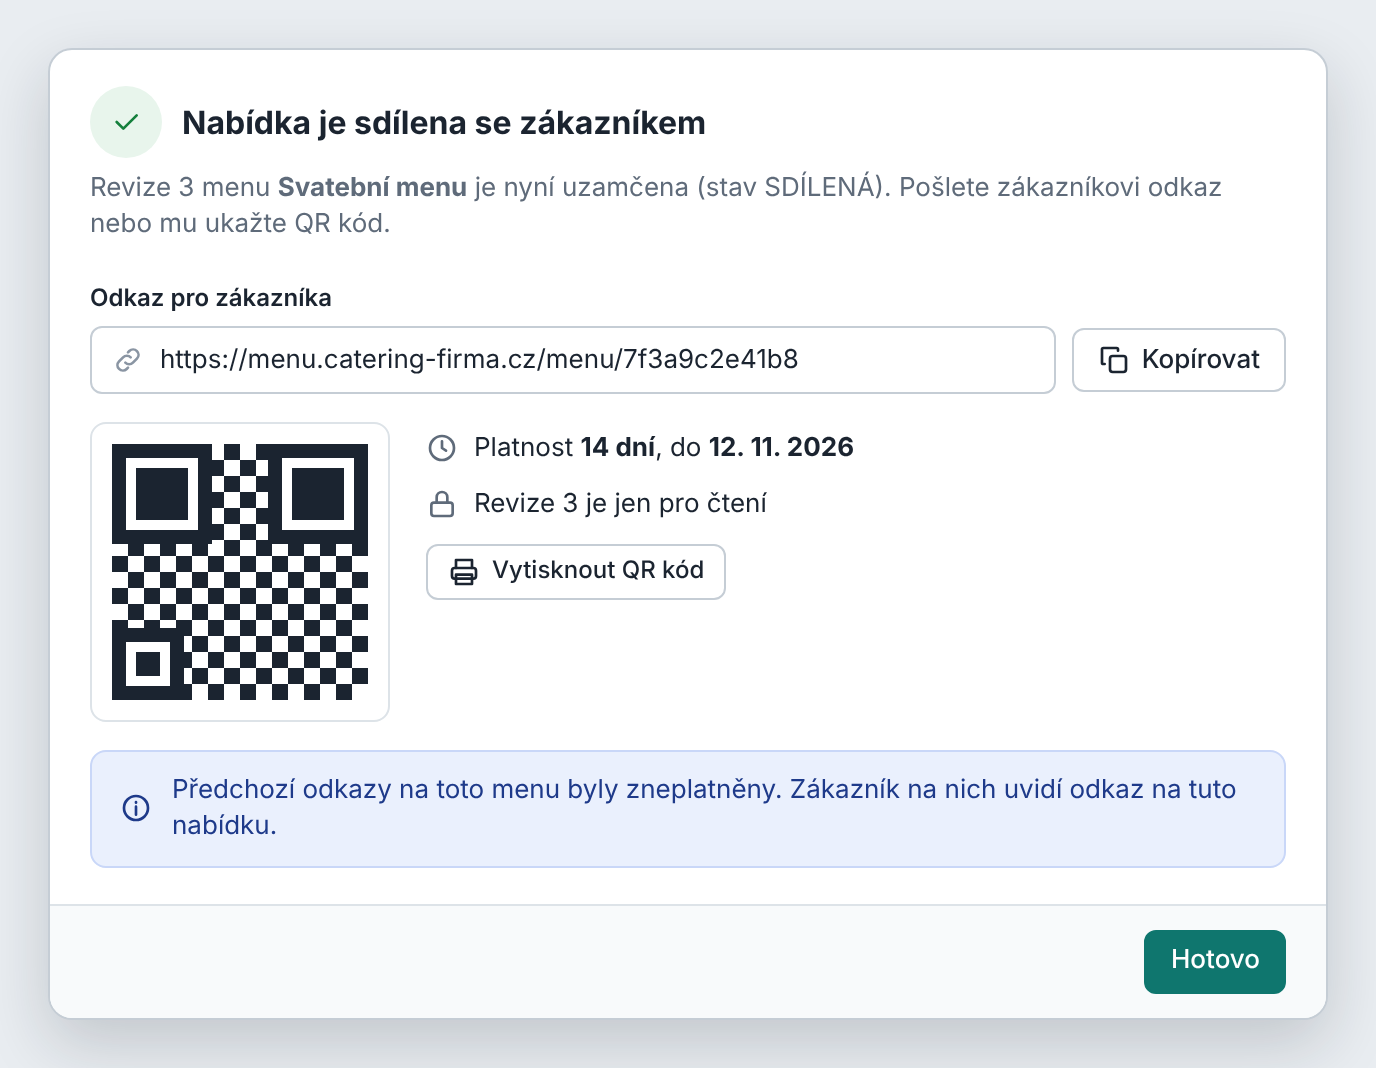
\includegraphics[width=0.66\textwidth]{ui-share.png}
  \caption{D6 -- Dialog sdílení nabídky}
  \label{fig:d6}
\end{figure}

Dialog se zobrazí po stisku \uv{Sdílet se zákazníkem} v editoru \odkaz{scr:D4}{D4} (\odkaz{uc:11:1}{UC11/1}--2). Nadpis potvrzuje, že revize byla sdílena a uzamčena.

Dialog obsahuje odkaz s tlačítkem pro zkopírování do schránky, datum platnosti a QR kód, který lze zákazníkovi ukázat nebo vytisknout (\odkaz{uc:11:3}{UC11/3}). Modrý pruh upozorňuje, že starší odkazy na totéž menu přestaly platit. Tlačítko \uv{Hotovo} dialog zavře a vrátí se do editoru \odkaz{scr:D4}{D4}.

\phantomsection\label{scr:D7}
\subsubsection*{D7 -- Správa uživatelů (\ucref{16})}

\begin{figure}[H]
  \centering
  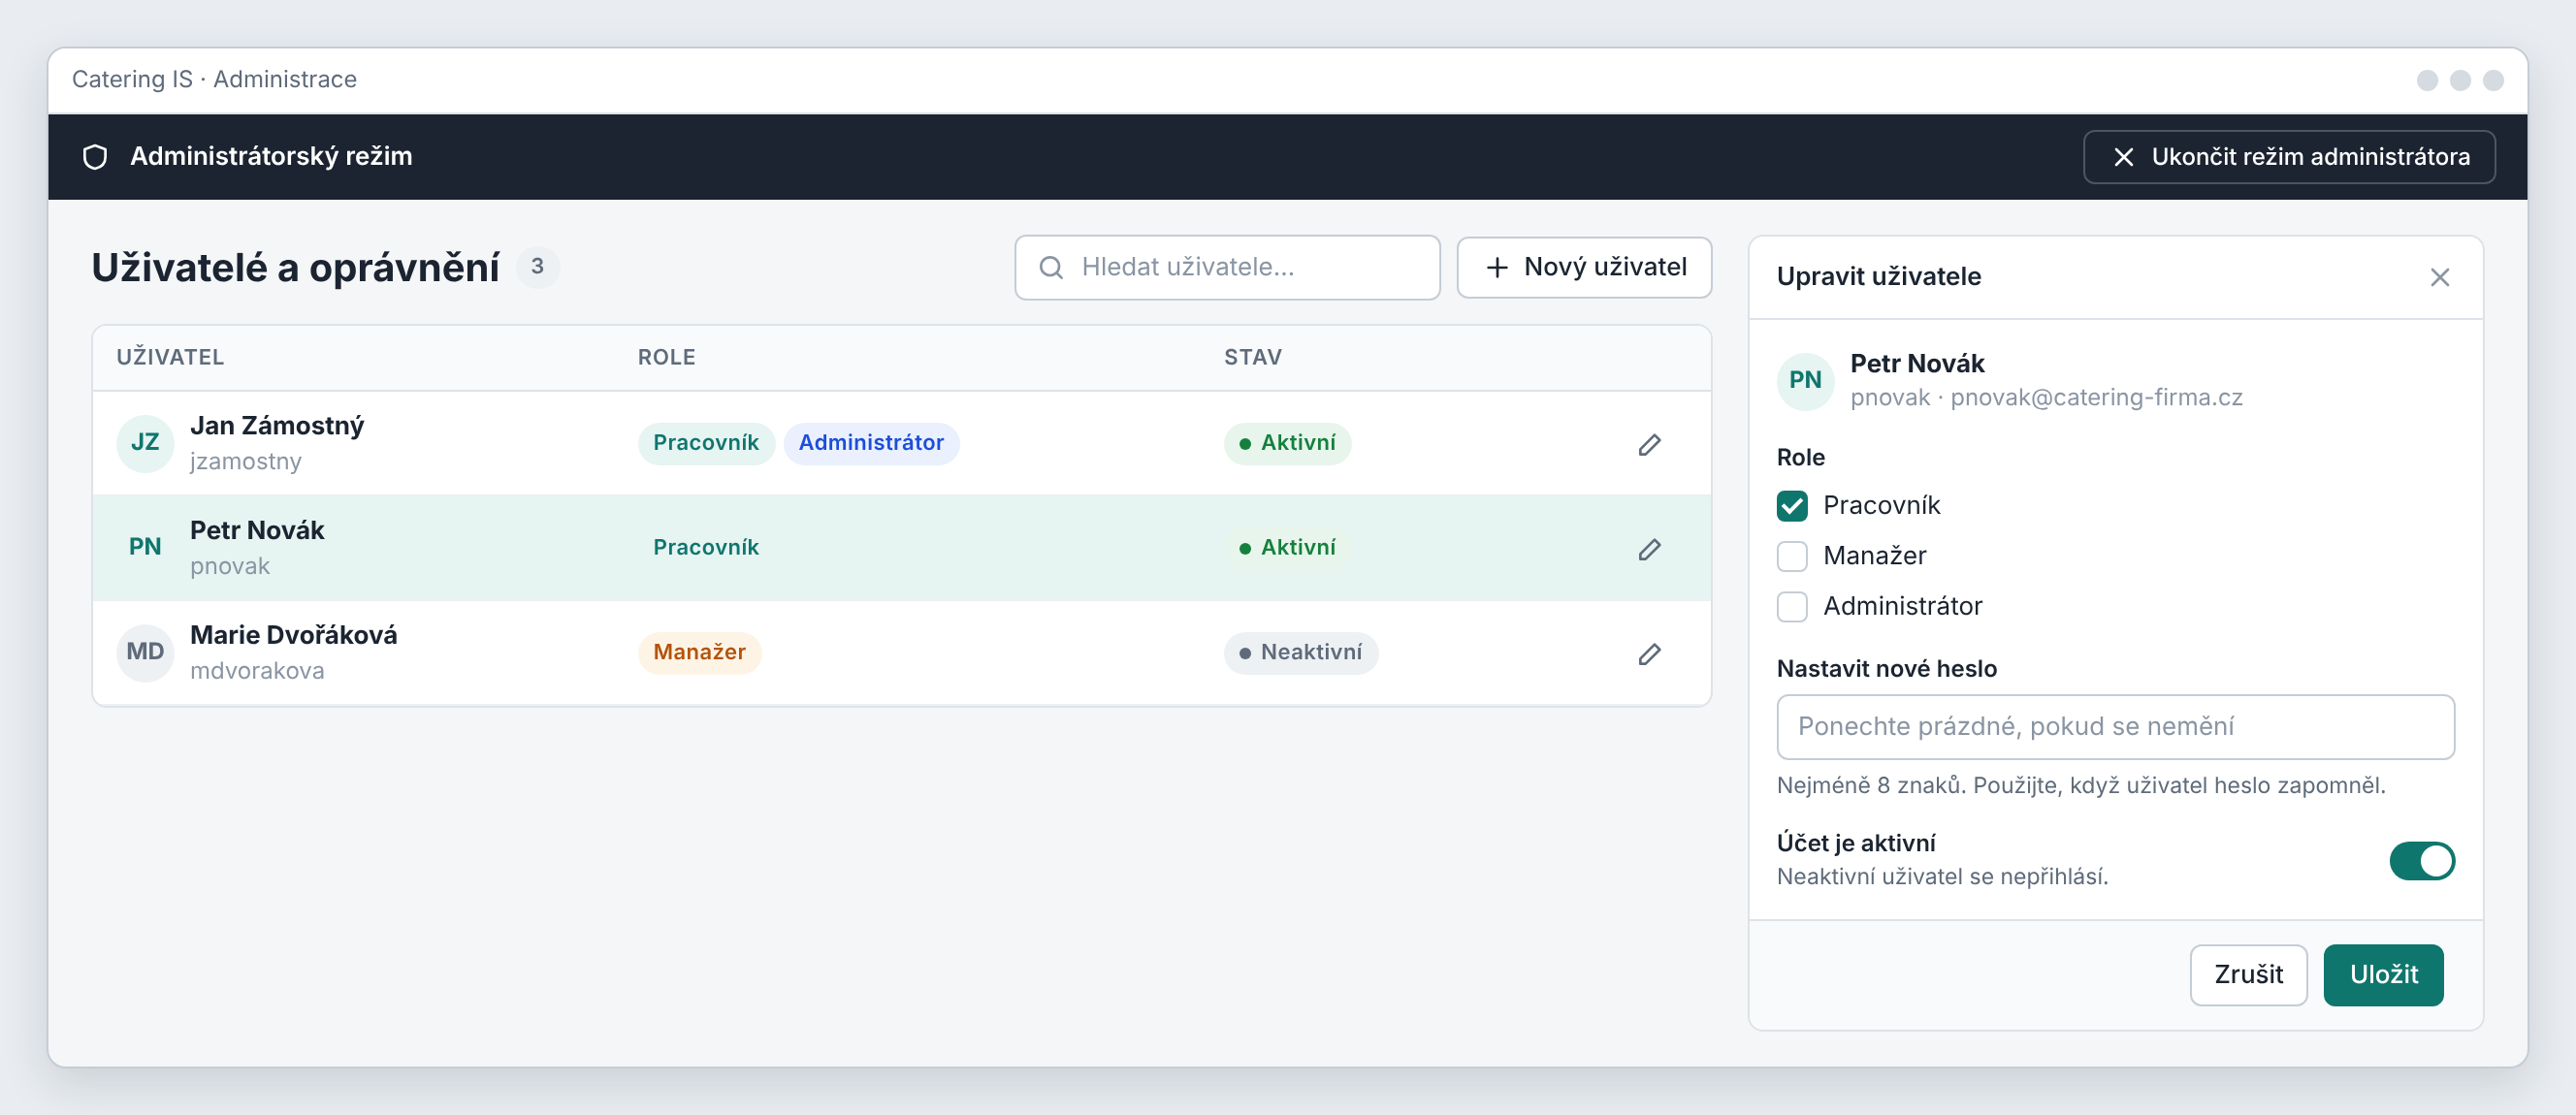
\includegraphics[width=\textwidth]{ui-users.png}
  \caption{D7 -- Správa uživatelů a oprávnění v administrátorském režimu}
  \label{fig:d7}
\end{figure}

Obrazovka se zobrazí po přepnutí do administrátorského režimu v okně \odkaz{scr:D1}{D1} (\odkaz{uc:16:1}{UC16/1}--2). Administrátor bez role pracovníka ji uvidí rovnou po přihlášení. Tmavý pruh nahoře trvale připomíná, že aplikace je v administrátorském režimu, a obsahuje tlačítko \uv{Ukončit režim administrátora}, které vrátí aplikaci do okna \odkaz{scr:D1}{D1} (u administrátora bez role pracovníka aplikaci ukončí).

Tabulka ukazuje uživatele s rolemi a stavem účtu ve formě štítků.

Tlačítko \uv{Nový uživatel} otevře vpravo formulář s uživatelským jménem, celým jménem, e-mailem, heslem a rolemi (\odkaz{uc:16:3}{UC16/3}). Po stisku \uv{Uložit} systém údaje ověří a uloží (\odkaz{uc:16:4}{UC16/4}--5). Chybné údaje nebo obsazené uživatelské jméno se ohlásí přímo u příslušného pole (\odkaz{uc:16:4.1}{UC16/4.1}--4.3).

Tlačítko s tužkou u řádku otevře zkrácený formulář vybraného uživatele, jak ukazuje obrázek~\ref{fig:d7} (\odkaz{uc:16:6}{UC16/6}). Jméno a e-mail jsou v něm jen pro čtení.

Měnit lze role, přepínač \uv{Účet je aktivní}, kterým se účet deaktivuje, a nepovinné pole \uv{Nastavit nové heslo} pro uživatele, který heslo zapomněl. Po stisku \uv{Uložit} systém ověří, že má nové heslo alespoň 8 znaků, a změnu uloží (\odkaz{uc:16:7}{UC16/7}--8).

Při pokusu odebrat posledního administrátora se zobrazí chybové okno a formulář vrátí původní hodnoty (\odkaz{uc:16:7.2}{UC16/7.2}--7.3).

\phantomsection\label{scr:D8}
\subsubsection*{D8 -- Potvrzení smazání (\ucref{19})}

\begin{figure}[H]
  \centering
  
\includegraphics[width=0.6\textwidth]{ui-delete.png}
  \caption{D8 -- Potvrzení smazání vybraných položek}
  \label{fig:d8}
\end{figure}

Dialog se zobrazí po stisku \uv{Smazat} v okně \odkaz{scr:D1}{D1}. Nadpis uvádí počet položek, pod ním je upozornění, že akci nelze vrátit, a seznam vybraných položek.

Položky se smažou až po stisku červeného tlačítka \uv{Smazat}. \uv{Zrušit} dialog zavře a nic nesmaže.

Neprázdnou složku a menu s aktivním odkazem pro zákazníka nelze smazat. Systém v tom případě nesmaže žádnou z vybraných položek a v chybovém okně uvede důvod.

\subsection{Webové rozhraní}

Webové stránky jsou navrženy nejprve pro mobilní telefon, protože zákazník odkaz často otevře z e-mailu nebo naskenuje QR kód. Na širší obrazovce se obsah zobrazí ve sloupci uprostřed stránky o šířce nejvýše 640 px.

\clearpage
\phantomsection\label{scr:W1}
\subsubsection*{W1 -- Sdílená nabídka (\ucref{11}, část zákazníka)}
\begin{figure}[H]
  \centering
  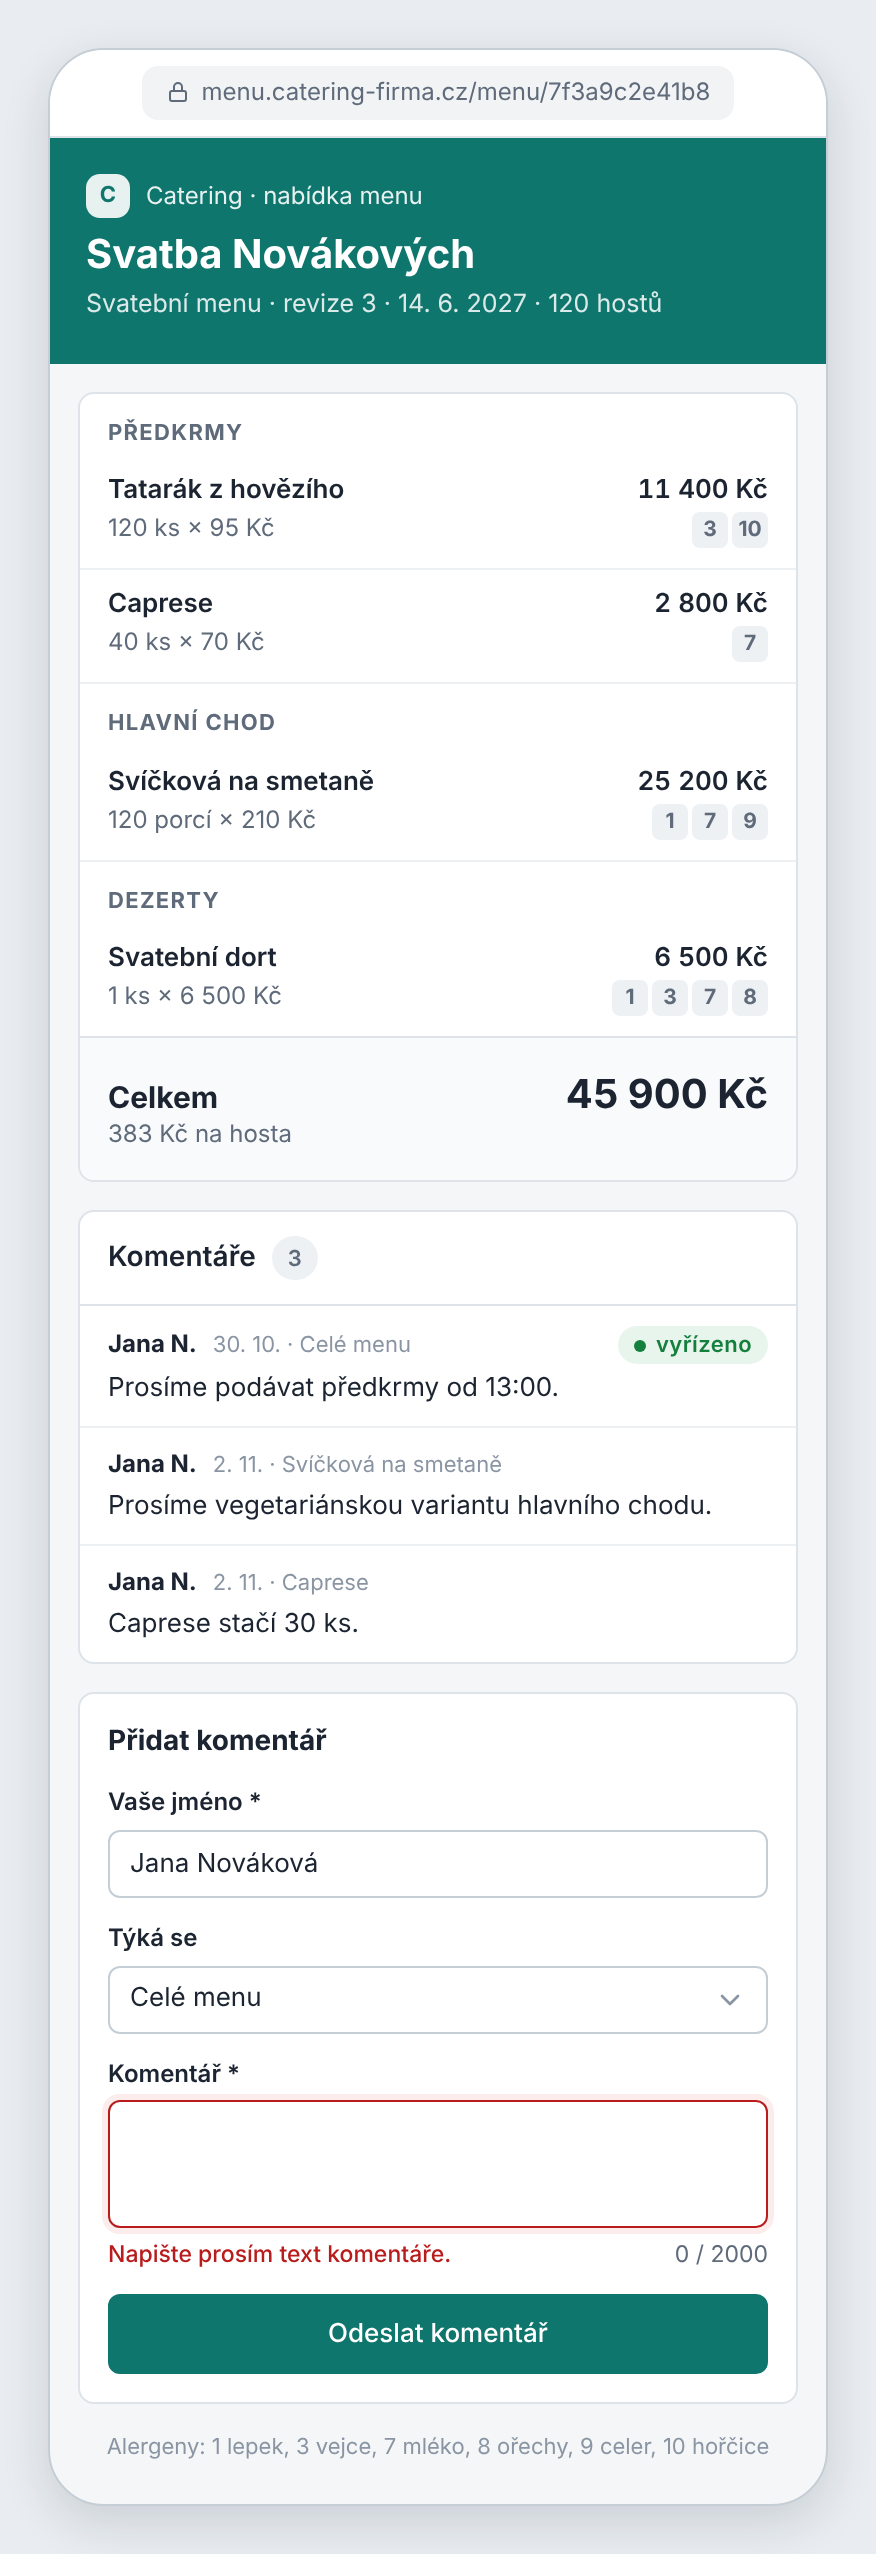
\includegraphics[height=0.8\textheight]{ui-web-menu.png}
  \caption{W1 -- Webová stránka se sdílenou nabídkou na mobilním telefonu}
  \label{fig:w1}
\end{figure}

Stránka se otevře z odkazu nebo QR kódu (\odkaz{uc:11:4}{UC11/4}--5, \ucref{12}).

V barevném záhlaví je název projektu, menu, číslo revize, datum akce a počet hostů. Pod ním jsou kategorie a položky. U každé položky je množství, jednotková cena, cena celkem a čísla alergenů, jejichž význam je vysvětlen dole na stránce. Celková cena a cena na hosta jsou zvýrazněny na konci menu.

Následuje seznam dosavadních komentářů s vyznačením vyřízených a formulář pro nový komentář: jméno, výběr položky (výchozí \uv{Celé menu}) a text (\odkaz{uc:11:6}{UC11/6}). Text komentáře má nejvýše 2000 znaků a pole ukazuje jejich počet (\odkaz{uc:11:7}{UC11/7}).

Po odeslání se stránka znovu načte se zeleným potvrzením nahoře a novým komentářem v seznamu (\odkaz{uc:11:7}{UC11/7}--8). Chybějící jméno nebo text se ohlásí červeně přímo u pole, jak ukazuje obrázek~\ref{fig:w1} (\odkaz{uc:11:7.1}{UC11/7.1}--7.3).

\phantomsection\label{scr:W2}
\subsubsection*{W2 -- Neplatný odkaz (\ucref{11}, alternativní průběh)}

\begin{figure}[H]
  \centering
  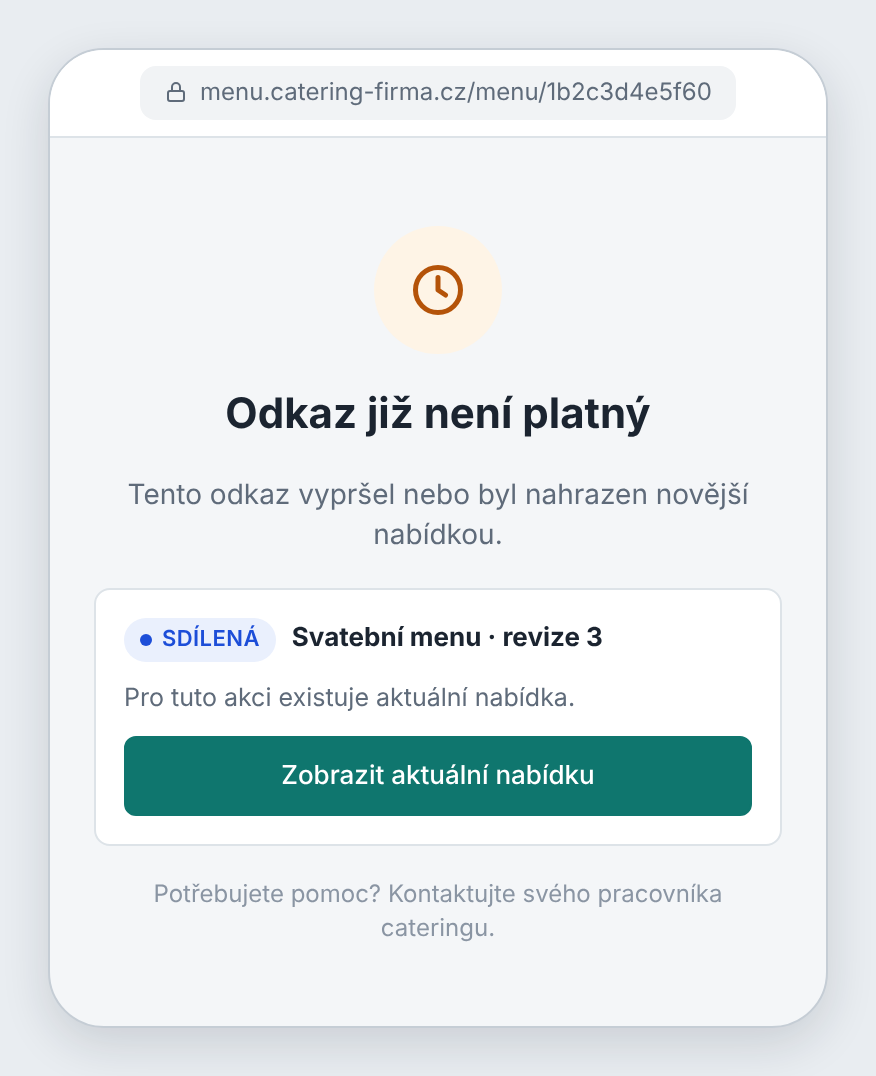
\includegraphics[width=0.36\textwidth]{ui-web-expired.png}
  \caption{W2 -- Stránka neplatného odkazu}
  \label{fig:w2}
\end{figure}

Stránka se zobrazí místo \odkaz{scr:W1}{W1}, pokud je odkaz prošlý nebo nahrazený (\odkaz{uc:11:5.1}{UC11/5.1}--5.3).

Existuje-li aktivní a neprošlý odkaz na totéž menu, stránka nabídne kartu s tlačítkem \uv{Zobrazit aktuální nabídku}, které vede na stránku \odkaz{scr:W1}{W1} s revizí tohoto odkazu (\odkaz{uc:11:5.4}{UC11/5.4}--5.6). Jinak karta chybí a zůstane jen doporučení kontaktovat pracovníka.

\subsection{Přechody mezi obrazovkami}

Označení obrazovek v tabulce jsou klikací odkazy na příslušné obrázky.

\begin{table}[H]
\centering
\small
\begin{tabularx}{\textwidth}{lXl}
\toprule
\textbf{Případ užití} & \textbf{Sekvence obrazovek} & \textbf{UI} \\
\midrule
\ucref{02} & \odkaz{scr:D1}{D1} $\rightarrow$ \odkaz{scr:D2}{D2} $\rightarrow$ \odkaz{scr:D1}{D1} (nová složka, nové menu, nahrání, stažení) $\rightarrow$ [\odkaz{scr:D3}{D3}] $\rightarrow$ \odkaz{scr:D1}{D1} $\rightarrow$ \odkaz{scr:D4}{D4} & desktop \\
\ucref{08} & \odkaz{scr:D1}{D1} $\rightarrow$ \odkaz{scr:D4}{D4} (úpravy, uložení) & desktop \\
\ucref{13} & \odkaz{scr:D4}{D4} $\rightarrow$ \odkaz{scr:D5}{D5} (zpracování) [$\rightarrow$ \odkaz{scr:D4}{D4} $\rightarrow$ \odkaz{scr:D5}{D5}] $\rightarrow$ \odkaz{scr:D4}{D4} & desktop \\
\ucref{11} & \odkaz{scr:D4}{D4} $\rightarrow$ \odkaz{scr:D6}{D6} $\rightarrow$ \odkaz{scr:D4}{D4} (pracovník), [\odkaz{scr:W2}{W2} $\rightarrow$] \odkaz{scr:W1}{W1} $\rightarrow$ \odkaz{scr:W1}{W1} po odeslání komentáře (zákazník) & desktop + web \\
\ucref{16} & \odkaz{scr:D1}{D1} $\rightarrow$ \odkaz{scr:D7}{D7} (seznam, formulář) $\rightarrow$ \odkaz{scr:D1}{D1} & desktop \\
\ucref{19} & \odkaz{scr:D1}{D1} $\rightarrow$ \odkaz{scr:D8}{D8} $\rightarrow$ \odkaz{scr:D1}{D1} & desktop \\
\bottomrule
\end{tabularx}
\caption{Sekvence obrazovek pro vybrané případy užití ([ ] = jen v alternativním průběhu)}
\label{tab:prechody}
\end{table}
